\setlength{\footskip}{8mm}

\chapter{Literature Review} 
\label{ch:literature-review}

\textit{This chapter begins with a review of the functional architecture of autonomous driving systems, coordinate systems, the PixHawk, and ROS coordinate conventions. To understand the SLAM process, the chapter also reviews SLAM, visual SLAM, ORB SLAM, and finally visual inertial ORB SLAM (VIORB).} 

\section{Software Architecture of Autonomous Driving Vehicles}
\label{section-name-in-literature-review}

\shortciteA{sbehere16t} splits the major components of the motion control part of autonomous driving systems into three main categories as shown in Figure \ref{fig:fav_automonous}. These categories are

\begin{itemize}
	\item Perception of the external environment in which the vehicle operates
	\item Decision making and control of vehicle motion with respect to the external environment that is perceived
	\item Vehicle platform manipulation, which deals mostly with sensing, control, and actuation of the vehicle, with the intention of achieving the desired motion.
\end {itemize}

Each category can be further broken down into several components. I describe each component in more details in the following sections.

\subsection{Perception}

\textit{Sensing components} sense the state of the vehicle and the state of the environment in which the vehicle operates. The \textit{sensor fusion component} considers multiple sources of information to construct a hypothesis or belief about the state of the environment. The \textit{localization component} determines the location of the vehicle with respect to a global map. The \textit{semantic understanding component} processes the sensor input and derives meaningful information from it. The \textit{world model component} holds the current estimate of the state of the external environment.

\subsection{Decision and Control}
The \textit{trajectory generation component} repeatedly generates a set of obstacle-free trajectories in the world coordinate system and picks an optimal trajectory from the set.  \textit{Energy management components} deal with energy management of the vehicle. \textit{Diagnosis and fault management} monitors the state of the overall system and its components. \textit{Reactive control components} are used for immediate responses to unanticipated stimuli from the environment. The \textit{vehicle platform abstraction component} refers to a minimal model of the vehicle platform. 

\subsection{Vehicle Platform Manipulation}

The \textit{platform stabilization component}'s task is to keep the vehicle platform in a controllable state during operation. \textit{Trajectory execution components} are responsible for executing the trajectory generated by the decision and control component. 

\begin{figure}
	\centering
	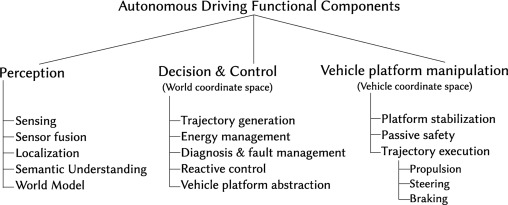
\includegraphics[width=5in]{figures/fav_autonomous_driving}
	\caption[FAV of Antonomous Driving System.]{\small 
		Functional architecture of an autonomous driving system. Reprinted from Behere (2016). }
	\label{fig:fav_automonous}
\end{figure}

\section{Coordinate Systems}

In this section I describe the different coordinate system conventions in use in robotic applications. 
	
\subsection{Earth Centric, Earth Fixed}

The earth-centered earth-fixed (ECEF) coordinate system, rotates with the Earth and has its origin at the center of the Earth. Refer to Figure~\ref{fig:coordinatesystem} (a) for a visualization. ECEF follows the right handed coordinate system convention. \citeA{coordinatesystem} describes ECEF as follows.

\begin{itemize}
	\item The origin is at the center of mass of the Earth, a point close to the Earth's center.
	\item The Z axis is on the line between the magnetic north and south poles, with positive values increasing northward (but not exactly coinciding with the Earth's rotational axis).
	\item The X and Y axes lie in the plane of the equator.
	\item The X axis passes through the point on the equator from 180 degrees longitude (negative) to the prime meridian (0 degrees longitude, positive).
	\item The Y axis passes through the point at 90 degrees west longitude along the equator (negative) to 90 degrees east along the equator (positive).
\end{itemize}

\subsection{Local tangent plane}

In the local tangent plane coordinate system, a position on the earth is fixed about the origin. There are two conventions as shown in Figure~\ref{fig:coordinatesystem} (b).

\begin{itemize}
	\item X=East, Y=North, Z=Up (ENU).
	\item X=North, Y=East, Z=Down (NED), which is commonly used in aviation, as the objects of interest usually lie before an aircraft (down or positive Z).
\end{itemize}

\begin{figure}%
	\centering
	\subfloat []{{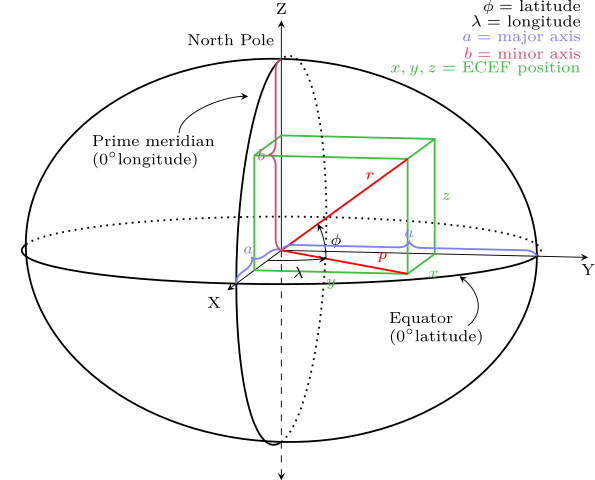
\includegraphics[width=3in]{figures/ECEF}}}%
	\subfloat []{{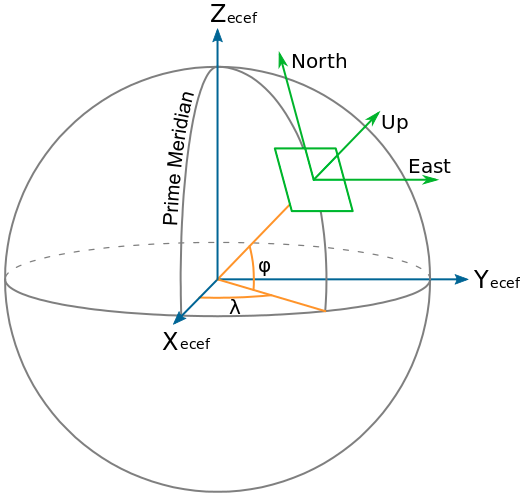
\includegraphics[width=3in]{figures/ENU_NED}}}%
	\caption[ECEF coordinate system]{\small Coordinate systems. (a) Earth centric, earth fixed (ECEF) coordinate system. (b) Local tangent plane coordinate systems. Reprinted from Krishnavedala. 
	}%
	\label{fig:coordinatesystem}%
\end{figure}

\subsection{PixHawk and ROS coordinate systems}

PixHawk follows the NED convention, whereas ROS follows the ENU convention. The conversion between these different conventions is handled automatically by MAVROS. To translate airframe-related data, a rotation of $180^{\circ}$ degrees is applied about the roll (X) axis. For local data, a $180^{\circ}$ rotation is applied about the roll (X) and $90^{\circ}$ rotation is applied about the yaw (Z) axes.

ROS has other reference frames as described by \shortciteA{rosrefframes}, shown in Figure \ref{fig:rosrefframes}.

\begin{itemize}
	\item The coordinate frame called \textit{base\_link} is rigidly attached to the mobile robot base. It can be attached in any arbitrary position or orientation.
	\item The coordinate frame called \textit{odom} is a world-fixed frame. The pose of a robot is continuous in this frame, but it can drift over time.
	\item The coordinate frame called \textit{map} is a world fixed frame, with Z-axis pointing upwards. 
	\item The coordinate frame called \textit{earth} is the origin of the ECEF frame.
\end{itemize}

\begin{figure}
	\centering
	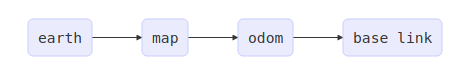
\includegraphics[width=5in]{figures/ros_rel_frames}
	\caption[Relation between ROS frames]{\small 
	Relationship between ROS frames. Reprinted from \shortciteA{rosrefframes}. }
	\label{fig:rosrefframes}
\end{figure}

\section{Simultanious Localization and Mapping}

\shortciteA{slamp1} describes the SLAM problem as a method by which a mobile robot can build a map of an environment and at the same time use this map to infer its location. In SLAM, both the trajectory of the platform and the location of all landmarks are estimated online without the
need for any a previous information of the location.

In probabilistic SLAM, the probability distribution, 
\begin{equation} \label{eq:slam1}
P({\bf x}_{k},{\bf m_k}\vert {\bf Z}_{0:k},{\bf U}_{0:k},{\bf x}_{0})
\end{equation}
has to be computed at any time instance $k$. The variables' meanings are as follows.
\begin{itemize}
	\item ${\bf x}_k$: the state vector describing the pose of the vehicle at time $k$.
	
	\item ${\bf u}_k$: the control vector applied at time $k - 1$ to drive the vehicle to state ${\bf x}_k$ at time $k$.
	
	\item ${\bf m}_i$: a vector describing the location of the $i^{th}$ landmark, whose true location is assumed time invariant.
	
	\item ${\bf z}_{ik}$: an observation taken from the vehicle of the location of the $i^{th}$ landmark at time $k$.
	
	\item ${\bf m_k}$: the set of all landmarks detected up to time $k$.
	
	\item ${\bf Z}_{0:k}$: the set of all observations up to time $k$.
	
	\item ${\bf U}_{0:k}$: the set of all control inputs up to time $k$.
	
\end{itemize}

The best estimate of ${\bf x}_k$ (pose) and ${\bf m}$ (map) at any time instance $k$ would be obtained by maximizing \ref{eq:slam1}.

The \textit{observation model} describes the likelihood of making an observation ${\bf z}_k$ when the vehicle location and landmark locations are known. The model is described in the form
\begin{equation}
P({\bf z}_{k}\vert {\bf x}_{k},{\bf m_k}).
\end{equation}

The \textit{motion model} for the vehicle can be described in terms of a probability distribution over state transitions in the form
\begin{equation}
P({\bf x}_{k}\vert {\bf x}_{k-1},{\bf u}_{k}).
\end{equation}

State transitions are assumed to be generated by to be a first-order Markov process that is independent of both the observations and the map. The next state ${\bf x}_k$ depends solely on the immediately preceding state ${\bf x}_{k-1}$ and the applied control ${\bf u}_k$.

Using the equations above, the pose of the vehicle and map can be estimated by standard two-step recursive (sequential) prediction (time-update) correction (measurement-update) form:

\textit{Time Update}
\begin{equation}
P({\bf x}_{k},{\bf m_k}\vert {\bf Z}_{0:k-1},{\bf U}_{0:k},{\bf x}_{0})= \int P({\bf x}_{k}\vert {\bf x}_{k-1},{\bf u}_{k}) \times P({\bf x}_{k-1},{\bf m_{k-1}}\vert {\bf Z}_{0:k-1}, {\bf U}_{0:k-1},{\bf x}_{0}){\rm d}{\bf x}_{k-1}
\end{equation}

\textit{Measurement Update}
\begin{equation}
P({\bf x}_{k},{\bf m_k}\vert {\bf Z}_{0:k},{\bf U}_{0:k},{\bf x}_{0}) = {P({\bf z}_{k}\vert {\bf x}_{k},{\bf m_k})P({\bf x}_{k}, {\bf m_k}\vert {\bf Z}_{0:k-1},{\bf U}_{0:k},{\bf x}_{0})\over P({\bf z}_{k}\vert {\bf Z}_{0:k-1},{\bf U}_{0:k})}
\end{equation}

An alternate way of expressing the problem is, if the location of the vehicle ${\bf x}_k$ is known at all times. The map can be estimated by computing
\begin{equation}
P({\bf m_k}\vert {\bf X}_{0:k},{\bf Z}_{0:k}, {\bf U}_{0:k}).
\end{equation}

If, on the other hand, the landmark locations are known, the vehicle can be localized by computing
\begin{equation}
P({\bf x}_k\vert {\bf Z}_{0:k},{\bf U}_{0:k}, m_k)
\end{equation}

\section{Visual SLAM}
Visual SLAM uses images from one or more cameras for observation of the landmarks (usually 3D points). \shortciteA{taketomi2017} report on a survey of Visual SLAM algorithms published between 2010 and 2016. Visual SLAM can be classified into feature based and direct methods. \textit{Feature based} methods extract features from the input image and use those features as observations.

Feature based vSLAM cannot function well in environments that are, feature-less or have weak texture. Furthermore, the point clouds produced by feature based methods are sparse. Some of the important feature based vSLAM algorithms are

\begin{itemize}
	\item Parallel Tracking and Mapping (PTAM) \cite{4538852}.
	\item ORB SLAM \cite{7219438}.
	\item ORB SLAM2 \cite{7946260}.
	
\end{itemize}


\textit{Direct methods} for vSLAM takes the whole image for tracking and mapping and produce dense point clouds. Some of the direct(featureless) vSLAM algorithms are

\begin{itemize}
	\item Dense Tracking and Mapping (DTAM) \cite{6126513}.
	\item Large-Scale Direct SLAM (LSD SLAM) \cite{Engel2014LSDSLAMLD}.
\end{itemize}

vSLAM algorithms have three basic modules:
\begin{enumerate}
	\item Initialization: Global coordinate system is defined, and an initial map is constructed from the environment.
	\item Tracking: Landmarks with known map associations are tracked to estimate the pose of the camera in the global coordinate system.
	\item Mapping: Map is expanded when the camera observes previously unexplored regions.
\end{enumerate}

Other modules that are used to increase the stability and accuracy of vSLAM are
\begin{enumerate}
	\item Re-localization: If tracking is lost, re-localization helps in recovering the camera's pose in the global coordinate system.
	\item Global map optimization: The reconstructed map accumulates estimation error over time as the camera is moved. This module minimizes the accumulated error. Loop closing can help reduce the accumulated error if a region that has been observed is encountered again. Bundle adjustment optimizes the map and the camera poses to minimize the total accumulated reprojection.
\end{enumerate}


The limitation of vSLAM algorithms, which can hinder their usage in practical applications, as mentioned by \shortciteA {taketomi2017} are

\begin{itemize}
	\item Purely rotational movement: Monocular vSLAM cannot map new points under purely rotational movement, as no disparity can be observed for triangulation.
	\item Map initialization: To get an accurate initial map, the baseline between the two images used for initialization should be large, and the number of features should be large. 
	\item Estimating Intrinsic camera parameters: The camera to be used must be calibrated beforehand, and the  camera matrix $K$ and the distortion coefficients $d_1$, $d_2$, $p_1$, and $p_2$ have to be known.
	\item Rolling shutter distortion: Cheap cameras have rolling shutter, which means that the same image may contain different regions captured at slightly different times from slightly different camera poses, making resulting triangulations inconsistent. 
	\item Scale Ambiguity: In monocular vSLAM, the absolute scale is unknown. Hence the pose and map generated may not be at the same scale as the actual world coordinates.
\end{itemize}




\subsection{ORB SLAM}

ORB SLAM \cite{7219438} is a monocular feature-based vSLAM algorithm. It uses ORB feature detectors for both mapping and tracking. It has three threads running in parallel for tracking, local mapping, and loop closing as shown in Figure \ref{fig:orb_slam1}.

\textit{Automatic Map Initialization} is done by finding corresponding ORB features in an initial frame $F_c$ and a reference frame $F_r$. In parallel threads, a homography ${\bf H}_{cr}$ and fundamental matrix ${\bf F}_{cr}$ are calculated. At each iteration, a score $S_M$ is computed. The model (homography or fundamental matrix) with the highest score is chosen. If there are no candidate models, the process is repeated again. For a planar scene, the homography model will be chosen, otherwise fundamental matrix model will be chosen. In the case of a homography, eight motion hypotheses are retrieved. The solution with most points seen in parallax in front of both the camera with low re-projection error is chosen. In the case of the fundamental matrix, it is first converted into an essential matrix using the calibration matrix $K$, then four motion hypotheses are considered. Each solution is evaluated in the same way as the homography. After initialization bundle adjustment is done to refine the initial reconstruction.

In the \textit{tracking} threads images are divided into cells, and at least 5 features per cell are extracted using the ORB detector. Uniform/low-contrast cells require the number of features per cell to be adapted. If tracking was successful for the previous frame, a constant-velocity motion model is used to predict the camera pose and perform a guided search for the map points tracked in the last frame. If the motion model is violated, a wider search is performed for the map points around their positions in the last frame. The pose is finally optimized with the found correspondences. If tracking is lost, the frame is converted into a bag of words, and the method queries the recognition database for keyframe candidates for global relocalization. After getting an estimation of the camera pose and an initial set of feature matches, the map is projected into the frame and more map-to-point correspondences are searched for. The camera pose is then optimized again with all the map points found in the frame. Finally, a decision whether to add the current frame as a new keyframe is taken. To insert a new keyframe, more than 20 frames must have passed from the last global relocalization, and local mapping should be idle, or more than 20 frames must have passed from the last keyframe insertion, with the current frame tracking at least 50 points and less than 90\% of the points in the reference keyframe.

In \textit{local mapping}, every new keyframe $K_i$ is analyzed. The covisibility graph is updated with $K_i$. A spanning tree linking $K_i$ with the keyframe having the most points in common with it is updated along with the bag-of-words representation of the keyframe. This will help in the data association for triangulating new points. Recent map points culling is done so that only a few outliers are present. New map points are created by triangulating ORB features observed in connected keyframes in the covisibility graph. To verify the points, we check for positive depth in both cameras, parallax, small reprojection error, and scale consistency. Local Bundle Adjustment is done to optimize the currently processed keyframe, along with the keyframes connected to it in the covisibility graph and all the map points seen by those keyframes. Outliers are discarded during the optimization. Local keyframe culling detects redundant keyframes and deletes them.

In the \textit{loop closing} thread, the last keyframe processed by the local mapping thread is taken and used to detect loops. Loop candidates detection is done by taking the bag of words vector of the current keyframe and comparing it for similarity with that of its neighbors, keeping the least score. Then all the keyframes with lower score are removed from the recognition database. All keyframes directly connected to the current keyframe are removed. Similarity transformation is calculated between the current frame and the loop candidate. If the similarity is supported by enough inliers, then a loop is accepted. Loop correction is done to fuse duplicated map points and insert new edges into the covisibility graph that attached to the loop closure. Finally, pose graph optimization over the essential graph is done to distribute the loop closing error along the graph. 


\begin{figure}
	\centering
	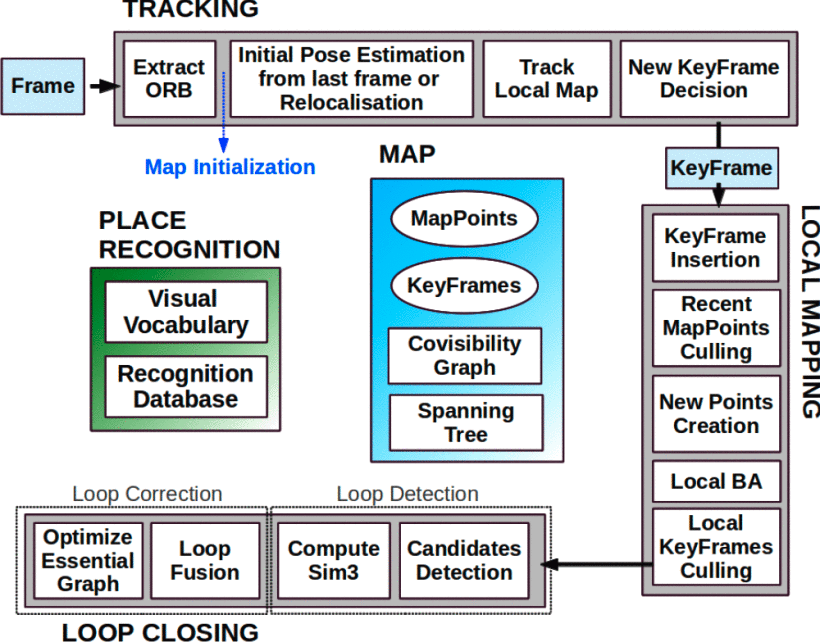
\includegraphics[width=5in]{figures/orb_slam1}
	\caption[ORB SLAM architecture]{\small 
		ORB SLAM system overview. Reprinted from \shortciteA{7219438}. }
	\label{fig:orb_slam1}
\end{figure}

\subsection{Visual Inertial ORB SLAM}

Visual Inertial ORB SLAM \shortcite{DBLP:journals/corr/Mur-ArtalT16} extends upon ORB SLAM by integrating a stream of IMU measurement to solve the scale ambiguity problem of monocular SLAM.

We write the IMU reference frame as ${\bf B}$, and assume camera and IMU are rigidly attached and the transformation ${\bf T}_{CB}$ between the two frames can be obtained through calibration.

Rotation, and transformations with subscripts $AB$ indicates "from $B$ to $A$". Position, and velocity with prefix subscript $A$ and postfix subscript $B$ indicates "$B$ with respect to $A$".

\begin{equation}
{\bf T}_{CB} = \left [
\begin{tabular}{ccc}
${\bf R}_{CB}$ & $\vert$ & $_C{\bf p}_B$ \\
$0$ & & $1$ \\
\end{tabular}      
\right ] 
\end{equation}

The IMU orientation ${\bf R}_{WB}$, position ${_W}{\bf p}_{B}$ and velocity $_W{\bf v}_B$ in world reference frame $W$ at time $k+1$ can be predicted based on estimates at time $k$ and IMU measurements collected between time $k$ and $k+1$.

\begin{align} \mathbf {R}^{k+1}_{WB} = & \mathbf {R}^{k}_{WB} \, \text{Exp}\left(\left(\boldsymbol {\omega }^k_{B} - \boldsymbol {b}^k_g\right)\Delta t\right) \nonumber\\ _{W}\mathbf {v}^{k+1}_{B} = & {_{W}\mathbf {v}^{k}_{B}} + \mathbf {g}_{W} \Delta t + \mathbf {R}^{k}_{WB} \left(\boldsymbol {a}^k_{B} - \boldsymbol {b}^k_a\right)\Delta t \nonumber\\ _{W}\mathbf {p}^{k+1}_{B} = & {_{W}\mathbf {p}^{k}_{B}} + {_{W}\mathbf {v}^{k}_{B}} \Delta t + \frac{1}{2}\mathbf {g}_{W} \Delta t^2 + \frac{1}{2} \mathbf {R}^{k}_{WB} \left(\boldsymbol {a}^k_{B} - \boldsymbol {b}^k_a\right)\Delta t^2 \end{align}

Where
\begin{itemize}
	\item ${\boldsymbol \omega }_{B}$ is the angular velocity of the IMU, represented as a twist vector in $\mathbb{R}^3$. 
	\item $\boldsymbol {a}_{B}$ is the acceleration of the IMU
	\item $\boldsymbol{b}_a$ and $\boldsymbol {b}_g$ are the gradually varying bias of the accelerometer and gyroscope
	\item ${\bf g}_W$ is the acceleration due to gravity
\end{itemize}

Using IMU preintegration, 

\begin{align} \label{eq:imuslam1} \mathbf {R}^{i+1}_\mathtt {WB} = & \mathbf {R}^{i}_\mathtt {WB} \Delta \mathbf {R}_{i,i+1} \text{Exp}\left(\left(\mathbf {J}^g_{\Delta R}\mathbf {b}^i_g\right)\right) \nonumber\\ _\mathtt {W}\mathbf {v}^{i+1}_\mathtt {B} = & {_\mathtt {W}\mathbf {v}^{i}_\mathtt {B}} + \mathbf {g}_\mathtt {W} \Delta t_{i,i+1} \nonumber\\ &+ \mathbf {R}^{i}_\mathtt {WB} \left(\Delta \mathbf {v}_{i,i+1} + \mathbf {J}^g_{\Delta v} \mathbf {b}^i_g + \mathbf {J}^a_{\Delta v} \mathbf {b}^i_a\right) \nonumber\\ _\mathtt {W}\mathbf {p}^{i+1}_\mathtt {B} = & {_\mathtt {W}\mathbf {p}^{i}_\mathtt {B}} + {_\mathtt {W}\mathbf {v}^{i}_\mathtt {B}} \Delta t_{i,i+1} + \frac{1}{2}\mathbf {g}_\mathtt {W} \Delta t^2_{i,i+1} \nonumber\\ & + \mathbf {R}^{i}_\mathtt {WB} \left(\Delta \mathbf {p}_{i,i+1} + \mathbf {J}^g_{\Delta p} \mathbf {b}^i_g + \mathbf {J}^a_{\Delta p} \mathbf {b}^i_a\right) \end{align}

Preintegrations and Jacobians can be efficiently computed iteratively as IMU measurements arrive using \ref{eq:imuslam1}.

Hence we can localize the IMU using the stream of IMU measurement.

In \textit{tracking}, the IMU pose is estimated and the camera pose is predicted. The keypoint in the camera frame is matched with projected map points. Optimization is done on current frame by minimizing the feature reprojection error of all matched points and an IMU error term. 

In \textit{local mapping}, the keyframe N+1 is always included in the fixed window as it constrains the IMU states. The cost function is a combination of IMU error terms (6) and reprojection error terms. The local window in Visual-Inertial ORB-SLAM is retrieved by the transitory sequence of keyframes, while in ORB-SLAM is recovered using the covisibility graph.

In \textit{loop closing} the pose-graph optimization is performed on 6 Degrees of Freedom(DoF) instead of 7 DoF [23], because the scale is observed.  IMU model velocities are corrected by rotating them according to the corrected orientation of the associated keyframe.  BA in a parallel thread is done that optimizes all states, including velocities and biases. 

The \textit{IMU initialization} has the following steps:


\textit{Gyroscope bias estimation} can be done from the known orientation of two consecutive keyframes. A constant bias $b_g$ is optimized which minimizes the difference between gyroscope integration and relative orientation computed from ORB-SLAM, for all pairs of consecutive keyframes.

In \textit{scale and gravity approximation}, a scale  factor $s$ is computed which is used when transforming between camera $C$ and IMU $B$ coordinate systems.

In \textit{accelerometer bias estimation, and scale and gravity direction refinement}, the gravity magnitude $G$ and the accelerometer bias is combined.

In \textit{velocity estimation}, three consecutive keyframes are taken into consideration when calculating the velocity of the most recent keyframe.

In \textit{bias reinitialization after relocalization}, after the system relocalizes, gyroscope and accelerometer biases are re-estimated using 20 consecutive frames localized with only vision.



\FloatBarrier

